\documentclass{article}

\usepackage{graphicx}
\usepackage{tikz}
\usepackage{tikzsymbols}
\usetikzlibrary{calc,patterns,shapes.geometric}
\pagestyle{empty}
\usepackage[margin=0pt]{geometry}
\geometry{papersize={14in,12in}}

\def\centerarc[#1](#2)(#3:#4:#5){\draw[#1] ($(#2)+({#5*cos(#3)},{#5*sin(#3)})$) arc (#3:#4:#5);}

\begin{document}
	\begin{figure}
		\centering
		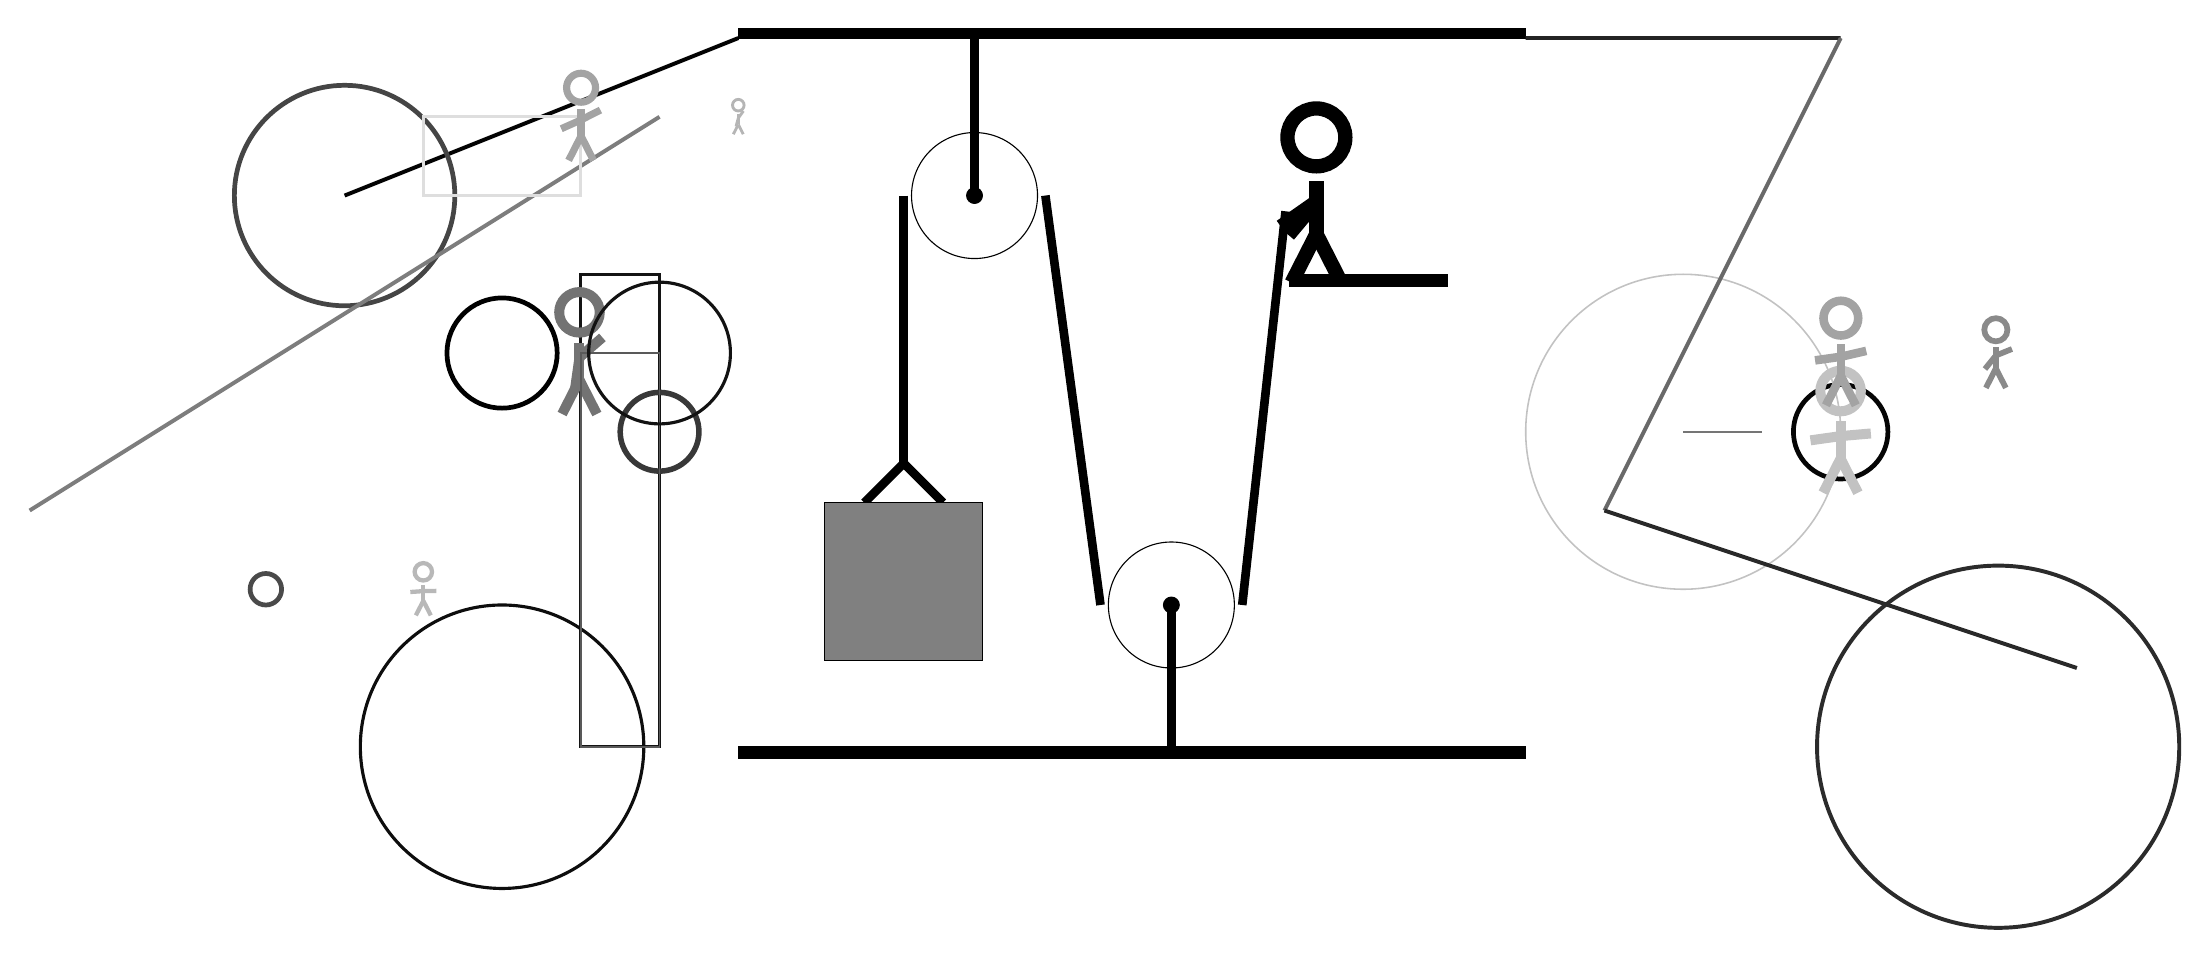
\begin{tikzpicture}
			%%%%% START %%%%%
			
			\draw[fill=black] (-2, 9) rectangle (8, 9.125);
			
			\draw (3.5, 1.8) circle (0.8);
			\draw[fill=black] (3.5, 1.8) circle (0.1);
			\draw[line width=1.1mm] (3.5, 1.8) -- (3.5, 0);
			
			\draw [line width=0.6mm, color=black!98](12, 4) circle (0.6);
			
			\node[line width=0.6mm, color=black!24] at (12, 4) {\Strichmaxerl[7][8][5]};
			\node[line width=0.5mm, color=black!29] at (-2, 8) {\Strichmaxerl[2][75][54]};
			\draw[line width=0.5mm, color=black!86] (8, 9) rectangle (12, 9);
			
			\draw[line width=0.2mm, color=black!54] (10, 4) rectangle (11, 4);
			\draw [line width=0.6mm, color=black!100](-5, 5) circle (0.7);
			\draw[line width=0.4mm, color=black!92] (-3, 6) rectangle (-4, 0);
			
			\draw [line width=0.7mm, color=black!78](-3, 4) circle (0.5);
			\draw[line width=0.5mm, color=black!99](-7, 7) -- (-2, 9);
			\draw [line width=0.4mm, color=black!95](-5, 0) circle (1.8);
			
			\draw [line width=0.6mm, color=black!73](-7, 7) circle (1.4);
			\node[line width=0.5mm, color=black!28] at (-6, 2) {\Strichmaxerl[3][4][1]};
			\node[line width=0.2mm, color=black!55] at (-4, 5) {\Strichmaxerl[7][82][41]};
			
			\draw [line width=0.2mm, color=black!24](10, 4) circle (2.0);
			\draw[line width=0.5mm, color=black!51](-3, 8) -- (-11, 3);
			\draw[line width=0.4mm, color=black!13] (-4, 8) rectangle (-6, 7);
			\draw[line width=0.5mm, color=black!59](9, 3) -- (12, 9);
			\draw[line width=0.2mm, color=black!65] (-4, 0) rectangle (-3, 5);
			\draw [line width=0.6mm, color=black!71](-8, 2) circle (0.2);
			\node[line width=0.4mm, color=black!46] at (14, 5) {\Strichmaxerl[4][51][22]};
			\node[line width=0.6mm, color=black!36] at (-4, 8) {\Strichmaxerl[5][24][27]};
			
			\draw [line width=0.5mm, color=black!83](14, 0) circle (2.3);
			\draw[line width=0.5mm, color=black!84](9, 3) -- (15, 1);
			\draw [line width=0.4mm, color=black!93](-3, 5) circle (0.9);
			\node[line width=0.2mm, color=black!36] at (12, 5) {\Strichmaxerl[6][8][13]};
			
			
			\draw (1, 7) circle (0.8);
			\draw[fill=black] (1, 7) circle (0.1);
			\draw[line width=1.1mm] (1, 9) -- (1, 7);
			
			\draw[line width=1.1mm](-0.4, 3.1) --  (0.1, 3.6) -- (0.6, 3.1);
			\draw[fill=black!50] (-0.9, 3.1) rectangle (1.1, 1.1);
			
			\draw[line width=1.1mm](0.1, 7) -- (0.1, 3.6);
			\centerarc[line width=1.1mm](1, 7)(180:0:0.9)
			\draw[line width=1.1mm](1.9, 7) -- (2.6, 1.8);
			\centerarc[line width=1.1mm](3.5, 1.8)(180:360:0.9)
			\draw[line width=1.1mm](4.4, 1.8) -- (4.95, 6.8);
			
			\node at (5.3, 7) {\Strichmaxerl[10][35][-130]};
			\draw[fill=black] (5, 6) rectangle (7, 5.85);
			
			\draw[fill=black] (-2, 0) rectangle (8, -0.15);
			
			%%%%% END %%%%%
		\end{tikzpicture}
	\end{figure}	
\end{document}